\documentclass[../main.tex]{subfiles}
\begin{document}
	
	\graphicspath{{AppendixA/}}
	\chapter{Supplementary Material on the CARDS method}
	\label{ch:cards-supp-info}
	
    \textit{The work in this Appendix is published in: Singh, S., 
    and Bowman, G.R., Quantifying allosteric communication via both concerted 
    structural changes and conformational disorder with CARDS. Journal of 
    Chemical Theory and Computation. 13:1507-1517, 2017. PMID: 28282132.}\cite{Singh:2017hha} 
	
	\section{Supplementary Methods}
        % \renewcommand{\thefigure}{\arabic{chapter}.S\arabic{figure}}
        % \setcounter{figure}{0}
        % \renewcommand{\theequation}{S\arabic{equation}}
        % \setcounter{equation}{0}
    \subsection{Molecular dynamics simulations}
        All simulations were carried out on GROMACS (version 5.1.1)\cite{Abraham:2015gj,VanDerSpoel:2005hz} using periodic boundary conditions in a dodecahedron with explicit water solvent. Simulations were carried out at 300K using the AMBER03\cite{Duan:2003gt} force field with the TIP3P water model\cite{Jorgensen:1983fl}. The starting conformations of wild-type apo and cAMP-bound CAP were generated by placing crystallographic structures (PDB ID: 4N9H and 1CGP respectively)\cite{Seok:2014cs,Schultz:1991uh} into separate dodecahedron boxes that extended 1.0 nm from the protein surface in any direction. Starting conformations fore the S62F variant were generated using the PyMol\cite{DeLano:2010wf} mutagenesis tool. Each system was then minimized independently with the steepest-descent algorithm until the maximum force fell below 1000 kJ/mol/min using a step size of 0.01nm and a cutoff distance of 1.2nm for the neighbor list, Coulomb interactions, and van der Waals interactions. For equilibration runs, all bonds were constrained with the LINCS algorithm\cite{Hess:2008fl} and virtual sites\cite{Feenstra:1999ue} were used to allow for a 4fs time step. As before, cut-offs of 1.0 nm were used for the neighbor list, Coulomb interactions, and van der Waals interactions. The Verlet cutoff scheme was used for the neighbor list, and Particle Mesh Ewald\cite{Essmann:1995gi} was employed for the electrostatics (with a grid spacing of 0.12nm, PME order 4, and tolerance 1e-5). The stochastic velocity rescaling (v-scale) thermostat\cite{Bussi:2007cs} was used to hold the temperature at 300K, and the Berendsen barostat\cite{Berendsen:1984fm} was used to bring the system to 1 bar pressure. For the production runs, the position restraint was removed and the Parrinello-Rahman barostat\cite{Parrinello:1981it} was employed. Conformations were stored every 10 ps. For each system, three 500ns runs were conducted totaling to 1.5$\mu$s of aggregate simulation time per system. 

        Dihedral angles were extracted using the MDTraj Library\cite{McGibbon:2015fv} (v. 1.7). Mappings were all drawn in PyMol (version 1.7)\cite{DeLano:2010wf}, and all figures were constructed in Inkscape (v. 0.48). 

    \subsection{Sensitivity analysis}
        We varied all the cutoff values employed in the CARDS algorithm to ensure the robustness of our results. Specifically, we varied the core width from 60° to 90°, the likelihood ratio cutoff from 1.5 to 5.0, and the neighbor distance cutoff from 2-6\AA. Fig. \ref{fig:cards-pearsonr-fig} demonstrates that the communication to the CBD does not change dramatically as these parameters are varied.

\section{Supplementary Figures}

    \begin{figure}[!htb] %Positioning code for figure
        \centering
        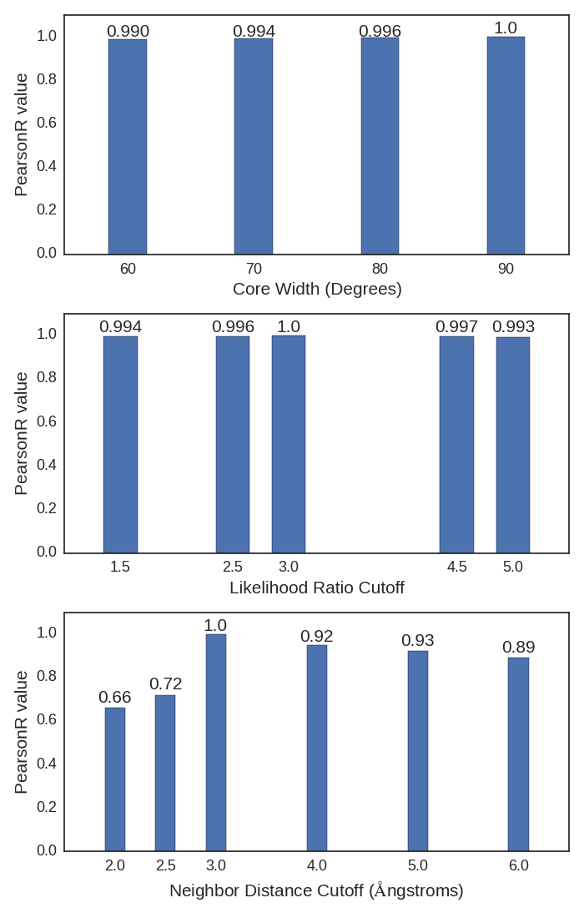
\includegraphics[width=4in]{suppfig1-pearsonr.png}
        \caption[CARDS sensitivity analysis]{Pearson Correlation Coefficients (PearsonR) between the CARDS results presented in the main text and those with varying A. the core width, B. the likelihood ratio cutoff, and C. the neighbor distance cutoff.}
        \label{fig:cards-pearsonr-fig}
    \end{figure} 

    \begin{figure}[!htb] %Positioning code for figure
        \centering
        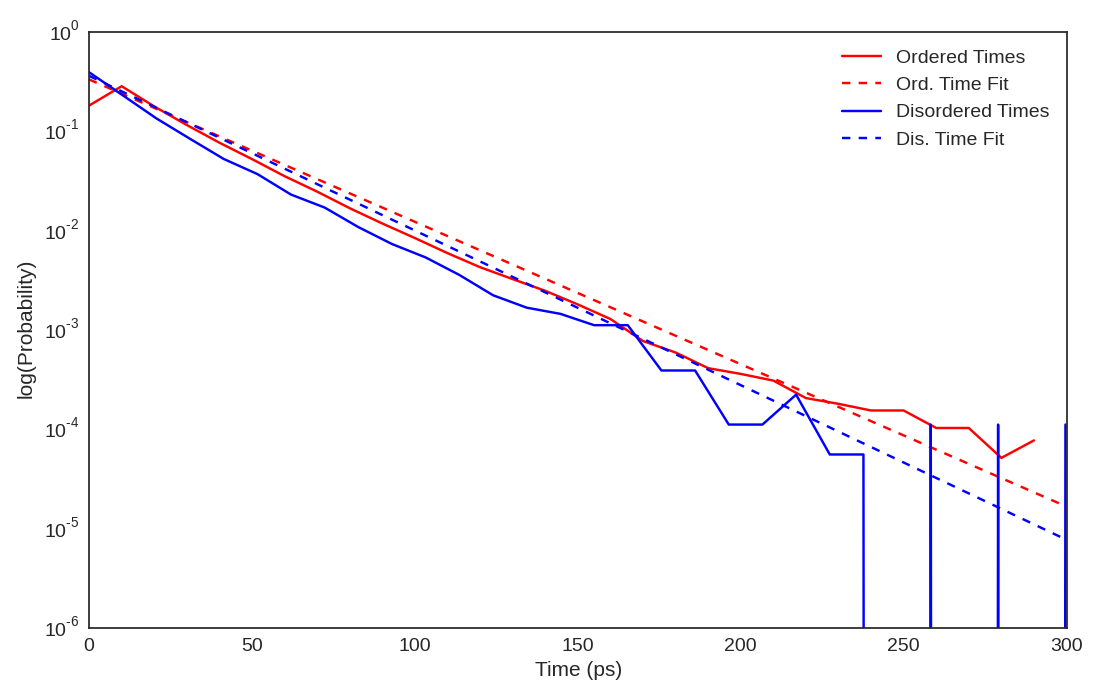
\includegraphics[width=4.5in]{suppfig2-timescale-dists.png}
        \caption[Distribution of ordered and disordered times for a single dihedral across a single simulation trajectory.]{The distribution of ordered and disordered times for a single dihedral across a single simulation trajectory. The solid lines represent the histogram of times extracted from the trajectory, while the dashed lines represent fits based on the average ordered ($\langle\tau_{ord}\rangle$) and disordered times ($\langle\tau_{dis}\rangle$).}
        \label{fig:cards-timescale-dists-fig}
    \end{figure} 

    \begin{figure}[!htb] %Positioning code for figure
        \centering
        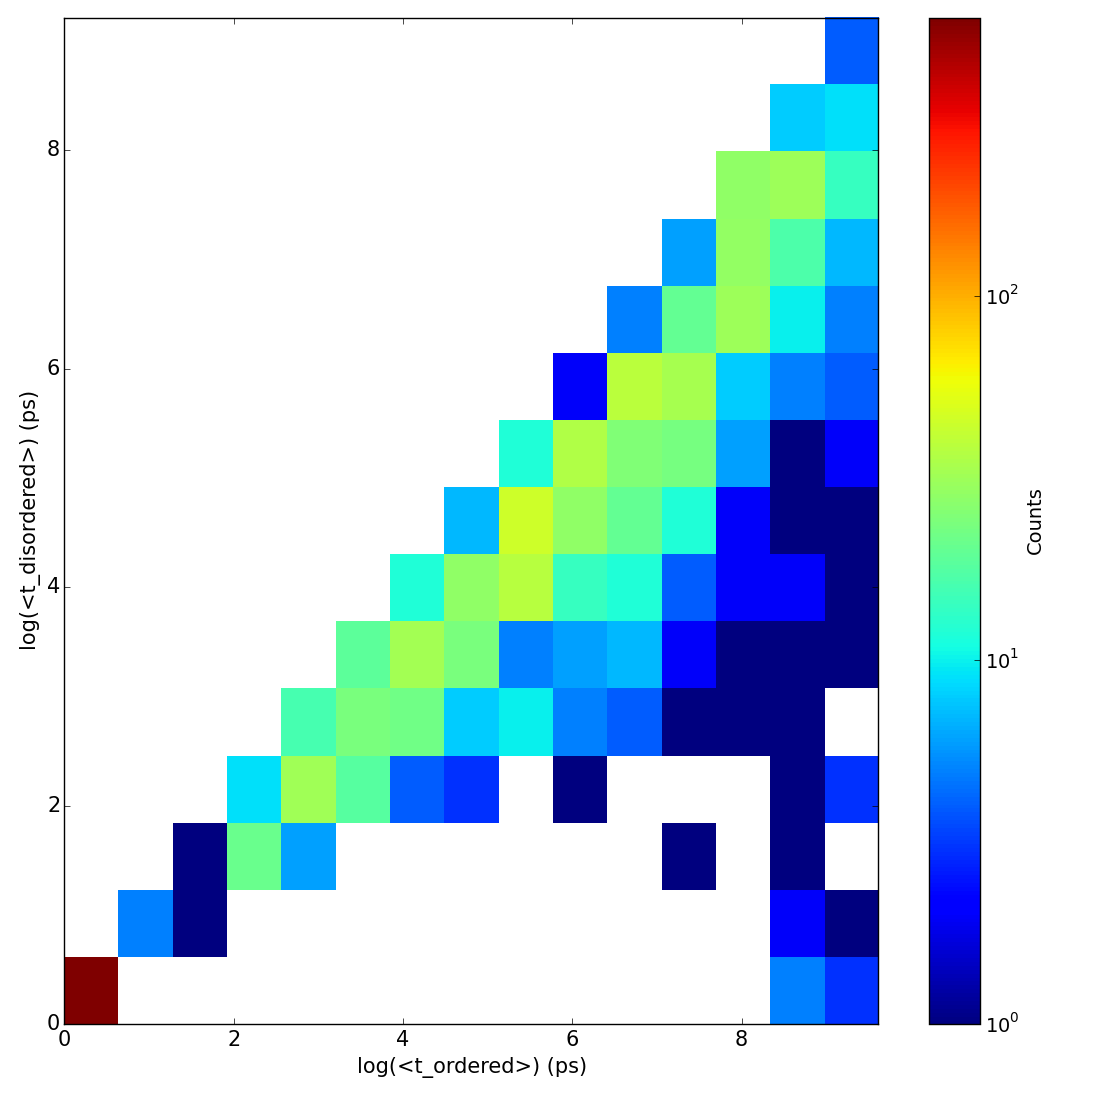
\includegraphics[width=4.5in]{suppfig3-avgtimes-2dhist.png}
        \caption[The average ordered and disordered times for CAP]{Two-dimensional histogram of the average ordered and disordered times ($\langle\tau_{ord}\rangle$ and $\langle\tau_{dis}\rangle$) for all dihedrals in CAP.}
        \label{fig:cards-avgtimes-2dhist-fig}
    \end{figure} 

    \begin{figure}[!htb] %Positioning code for figure
        \centering
        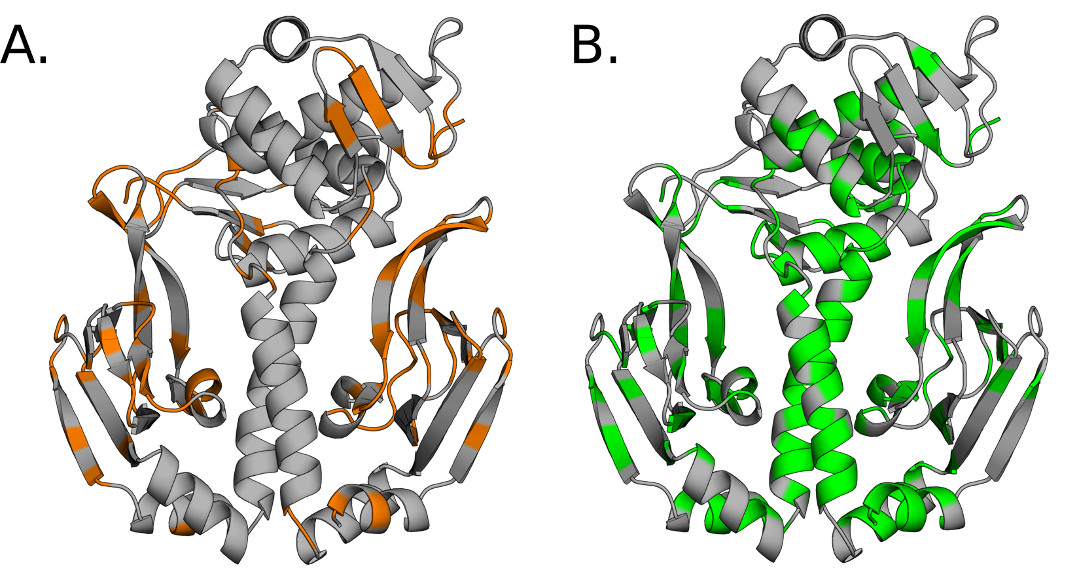
\includegraphics[width=4.5in]{suppfig4-disord-resis-cutoff.png}
        \caption[Residues with separable dihedrals into disordered regimes]{Residues with separable dihedrals into disordered regimes using a stricter threshold ($\langle\tau_{ord}\rangle \geq 5\times\langle\tau_{dis}\rangle$) A. Residues with at least one backbone dihedral that is capable of disorder-mediated communication (orange). B. Residues with at least one side-chain dihedral that is capable of disorder-mediated communication (green).}
        \label{fig:cards-disord-resis-cutoff}
    \end{figure} 

    \begin{figure}[!htb] %Positioning code for figure
        \centering
        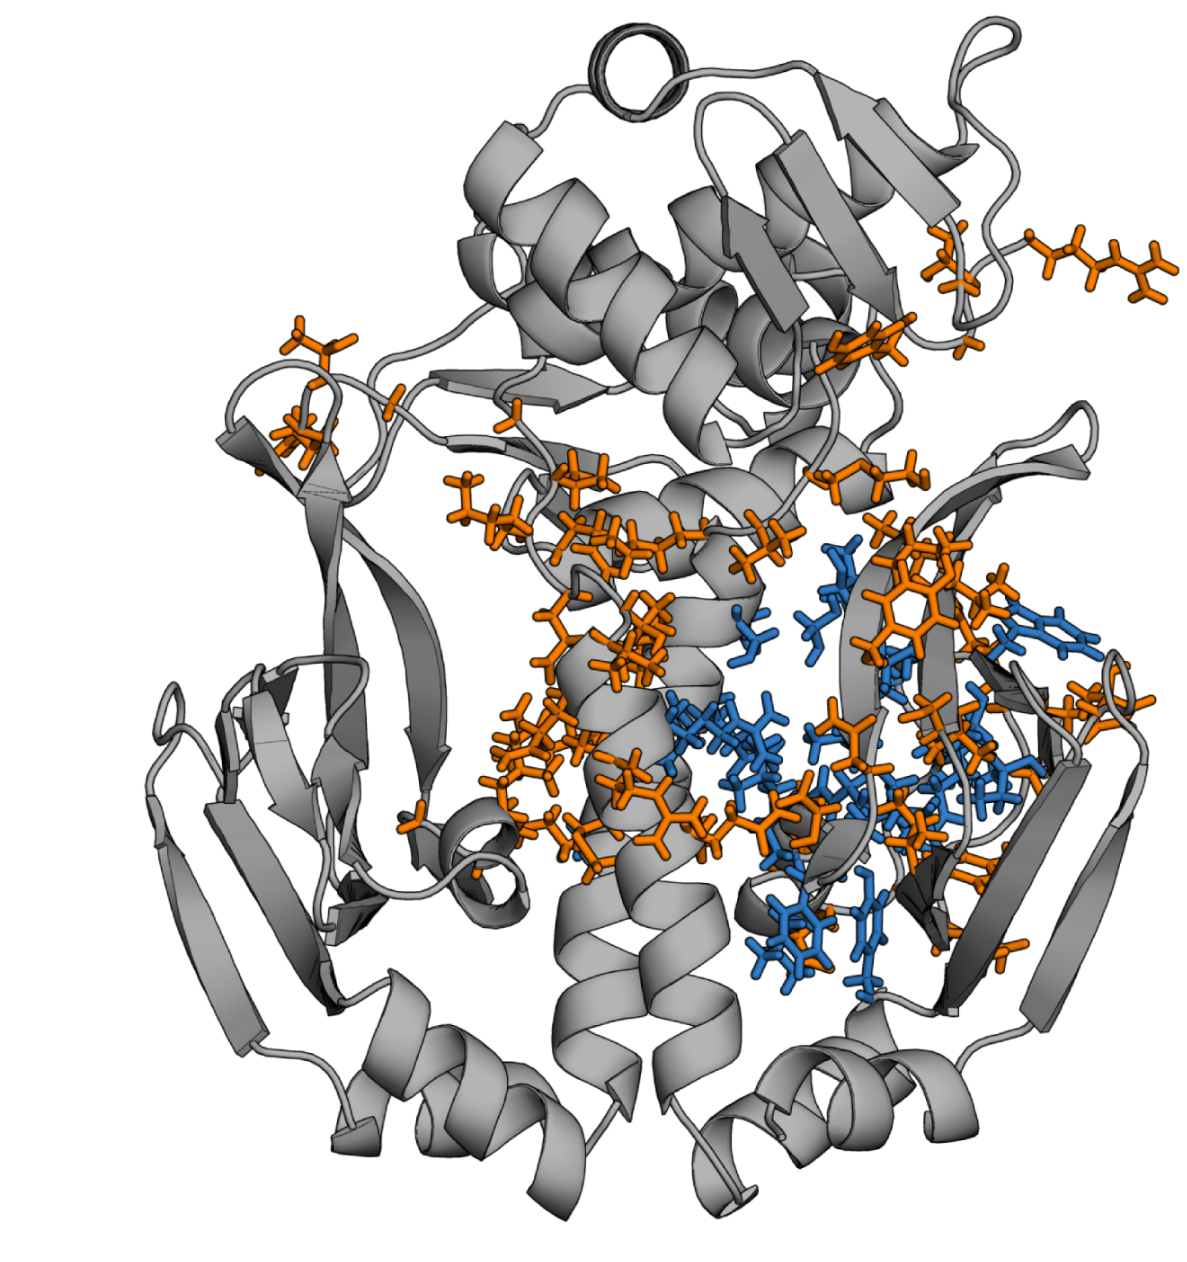
\includegraphics[width=4in]{suppfig5-top5percentresis.png}
        \caption[The top 5\% of residues (orange sticks) with disorder-mediated communication to the cAMP-binding pocket]{The top 5\% of residues (orange sticks) with disorder-mediated communication to the cAMP-binding pocket (blue sticks). Note that having disorder-mediated communication to the CBD does not preclude the possibility of also having structural communication.}
        \label{fig:cards-top5percentresis}
    \end{figure} 

    \begin{figure}[!htb] %Positioning code for figure
        \centering
        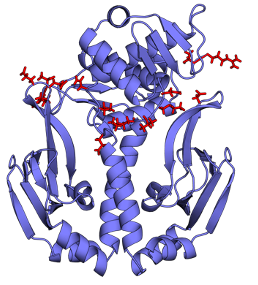
\includegraphics[width=2.5in]{suppfig6-top2percent-hubs.png}
        \caption[The top 2\% of backbone-side-chain hubs]{The top 2\% of backbone-side-chain hubs (sticks).}
        \label{fig:cards-top2percenthubs}
    \end{figure} 

    \begin{figure}[!htb] %Positioning code for figure
        \centering
        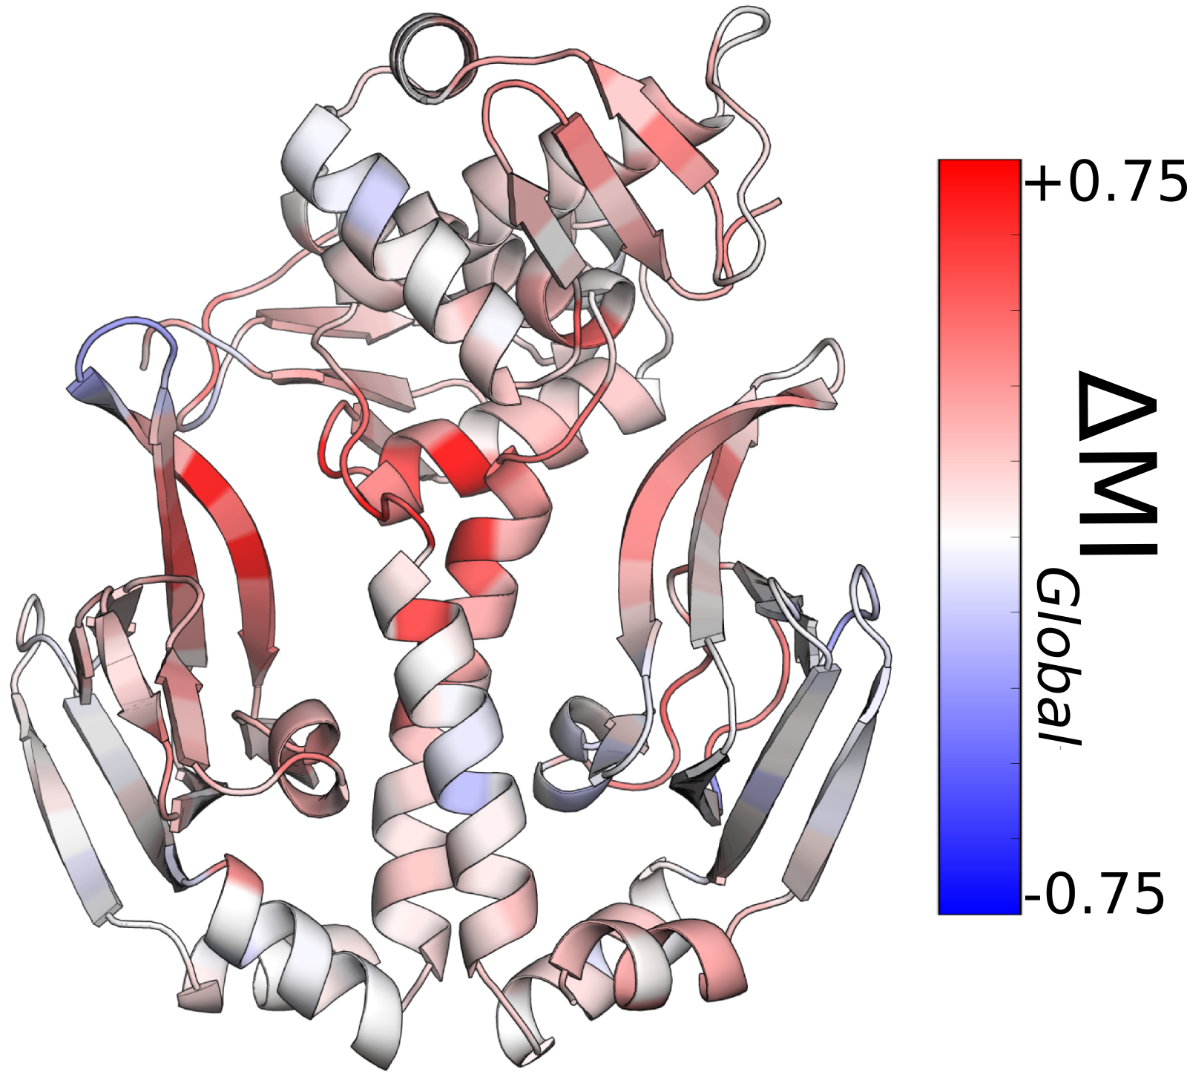
\includegraphics[width=3in]{suppfig7-deltaglobalMI.png}
        \caption[Change in global communication upon the S62F mutation.]{Change in global communication upon the S62F mutation. The color scale on the right shows the proportional change in global communication relative to the scale in Figure \ref{fig:cap-global-mi-fig} of the main text.}
        \label{fig:cap-deltaglobalMI}
    \end{figure} 
	
	
\end{document}